
%(BEGIN_QUESTION)
% Copyright 2010, Tony R. Kuphaldt, released under the Creative Commons Attribution License (v 1.0)
% This means you may do almost anything with this work of mine, so long as you give me proper credit

Suppose we have an Allen-Bradley MicroLogix 1000 controller connected to a pair of pushbutton switches and contactor controlling power to an electric motor as shown in this illustration:

$$\includegraphics[width=15.5cm]{i04663x01.eps}$$

This motor control system has a problem, though: the motor refuses to start when the ``Start'' pushbutton is pressed.  Examine the ``live'' display of the ladder logic program inside this Allen-Bradley PLC to determine what the problem is:

$$\includegraphics[width=15.5cm]{i04663x02.eps}$$

Identify at least two causes that could account for all you see here.

\underbar{file i04663}
%(END_QUESTION)





%(BEGIN_ANSWER)

\begin{itemize}
\item{} Contactor coil failed open
\item{} Wire connecting contactor coil to {\tt O:0/2} failed open
\item{} Wire connecting VAC-VDC terminal to DC COM terminal failed open
\item{} Wire connecting input switch ``commons'' to contactor coil failed open
\item{} Output channel {\tt O:0/2} defective on the PLC
\item{} 24 VDC power supply in the PLC is insufficient to power the contactor's coil
\end{itemize}

%(END_ANSWER)





%(BEGIN_NOTES)


%INDEX% PLC, relating I/O status to virtual elements (troubleshooting)

%(END_NOTES)


